\documentclass[12pt,utf8]{beamer}
\usepackage{graphicx}
\usepackage{xcolor}
\usepackage[ngerman]{babel}
\usepackage{wasysym}
\usepackage{Latex_Template/beamerthemeFOSSAG}

\title{Shells}
\subtitle{Alternativen zu Bash}
\author[N. Lenz]{Nicolas Lenz}
\institute[FOSS AG]{Free and Open Source Software AG\\Fakultät für Informatik}
\date{\today}

\begin{document}
	\titlepage
	\begin{frame}
		\frametitle{Inhalt}
		\begin{itemize}
			\item \textbf{osh}: Die Anfänge
			\item \textbf{sh}: Angestaubt
			\item \textbf{bash}: Solide und beliebt
			\item \textbf{zsh}: Leistungsfähig und anpassbar
			\item \textbf{BusyBox}: All-in-one
			\item \textbf{fish}: Freundlich und interaktiv
		\end{itemize}
	\end{frame}

	\begin{frame}
		\frametitle{Testfolie}
		\framesubtitle{Untertitel}
		Bla bla bla bla
		\begin{itemize}
			\item[\twonotes] Ja hallo
			\item[\twonotes] Tschau
			\begin{enumerate}
				\item was \texttt{geht}
				\item hallo
			\end{enumerate}
			\item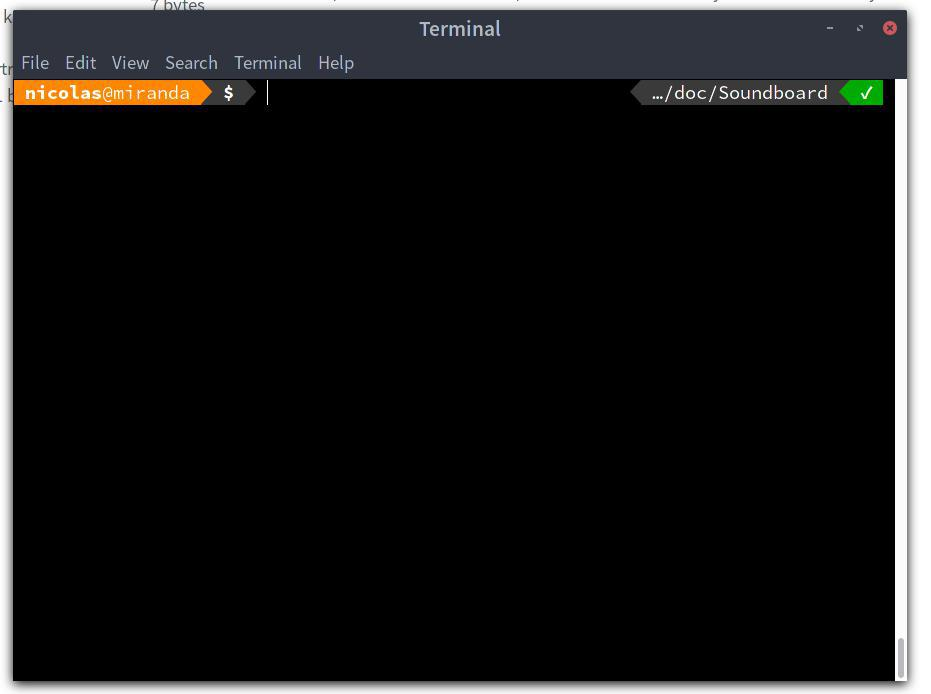
\includegraphics[scale=0.2]{res/test.jpg}
		\end{itemize}
	\end{frame}

	\begin{frame}
		\frametitle{Die Anfänge}
		\framesubtitle{Die Thompson-Shell}
		\begin{itemize}
			\item Erste UNIX-Shell, heute bekannt als \textbf{osh} für ``old shell``
			\item Verwendet in \textbf{UNIX} 1 bis 6 von 1971 bis 1975
			\item Führte Piping, einfache Kontrollstrukturen für Skripte und Wildcarding ein
		\end{itemize}
	\end{frame}

	\begin{frame}
		\frametitle{Die Anfänge}
		\framesubtitle{Die Bourne-Shell}
		\begin{itemize}
			\item Ursprünglich veröffentlicht \textbf{1977}
			\item Heute bekannt und immer noch genutzt als ``sh``
			\item 
		\end{itemize}
	\end{frame}
\end{document}